\documentclass[conf]{new-aiaa}
\usepackage[utf8]{inputenc}
\usepackage{graphicx}
\usepackage{amsmath}
\usepackage{booktabs}
\usepackage[version=4]{mhchem}
\usepackage{siunitx}
\usepackage{longtable,tabularx}
\usepackage{url}
\usepackage{subcaption}
\setlength\LTleft{0pt}
\graphicspath{{figures/}{./}}

\title{Time--Energy Trajectory Optimization for Lunar Rover Navigation}

\author{Martin Zhou and Sebastian Martinez}
\affil{Stanford University, Stanford, CA}

\begin{document}
\maketitle

\begin{abstract}
Autonomous lunar rovers must navigate cratered terrain while respecting mobility, power, and battery limits. This project presents a two-stage navigation pipeline that combines terrain-aware global planning with time--energy trajectory generation. The terrain layer converts elevation data into traversability and risk fields and computes a feasible high-level route with A$^\ast$. The trajectory layer uses a reduced-order rover dynamics and power model to produce a dynamically consistent route along the planner path. On a cratered lunar-terrain benchmark, the pipeline generates a feasible \SI{42.0}{km} traverse in approximately \SI{42.3}{h} while maintaining battery feasibility under the implemented power model.
\end{abstract}

\section{Introduction}
Sustained lunar exploration will require surface mobility systems that can move astronauts, cargo, science payloads, and infrastructure across regions that are not necessarily colocated with landing sites. NASA's Moon to Mars Architecture identifies long-term lunar surface exploration as a step toward sustained human-led science beyond Earth, and the Artemis Lunar Terrain Vehicle program is being developed to support crewed science operations near the lunar South Pole~\cite{nasa_moon_to_mars_architecture,nasa_ltv}. Future mobility systems must also support cargo relocation, surface infrastructure deployment, and autonomous or semi-autonomous operation to improve mission flexibility~\cite{nasa_lunar_mobility_drivers_2024}.

The lunar South Pole is a challenging domain for rover navigation because it contains heavily cratered terrain, dramatic topography, permanently shadowed regions, and highly illuminated ridges~\cite{lpi_south_pole_atlas}. NASA's lunar mobility analysis also notes that slopes greater than \SI{10}{deg} are common near the South Pole and that terrain, lighting, thermal conditions, power demand, and wheel--soil interaction strongly affect mobility-system design~\cite{nasa_lunar_mobility_drivers_2024}. Rover navigation must therefore account for terrain traversability, rover dynamics, mission time, power consumption, and battery feasibility.

This project addresses that setting with a modular planner--trajectory-generation pipeline. A terrain module converts an elevation map into slope, roughness, traversability, and risk information. A global A$^\ast$ planner computes a feasible high-level path, and a sequential convex programming (SCP) stage uses that path as a warm start for a constrained time--energy trajectory problem. This structure separates large-scale terrain avoidance from local dynamic and energy feasibility.

The formulation is motivated by prior work on energy-constrained rover routing and trajectory generation. Energy-aware planetary rover navigation has been formulated with explicit power limits and hybrid generation~\cite{hu2025rover}, while SCP has been developed as a practical framework for generating dynamically feasible trajectories~\cite{malyuta2022scvx}. For terrain-aware lunar path planning, prior work has also demonstrated the value of obstacle-aware planning in hazardous South Pole environments~\cite{feng2025southpole}.

\section{Problem Formulation}

\subsection{Rover Dynamics and Power Model}
The rover dynamics and power model is adapted from an energy-constrained planetary rover formulation that couples rover motion with translational, rotational, resistive, and baseline subsystem power terms~\cite{hu2025rover}. A reduced-order version is used here: the rover is represented in planar coordinates, the optimizer commands speed and heading, and the power model maps commanded motion and terrain resistance to battery depletion.

The discrete rover state is
\begin{equation}
    x_k = \begin{bmatrix} X_k & Y_k & E_k & v_k & \psi_k & \omega_k \end{bmatrix}^{\top},
\end{equation}
where $(X_k,Y_k)$ is planar position, $E_k$ is battery energy, $v_k$ is speed, $\psi_k$ is heading, and $\omega_k$ is yaw rate. The control input is
\begin{equation}
    u_k = \begin{bmatrix} v_k^{\mathrm{cmd}} & \psi_k^{\mathrm{cmd}} \end{bmatrix}^{\top}.
\end{equation}
For a time step $\Delta t$, the discrete kinematic update is
\begin{align}
    X_{k+1} &= X_k + \Delta t\, v_k^{\mathrm{cmd}}\cos\psi_k^{\mathrm{cmd}}, \\
    Y_{k+1} &= Y_k + \Delta t\, v_k^{\mathrm{cmd}}\sin\psi_k^{\mathrm{cmd}}, \\
    v_{k+1} &= v_k^{\mathrm{cmd}}, \\
    \psi_{k+1} &= \psi_k^{\mathrm{cmd}}, \\
    \omega_{k+1} &= \frac{\psi_k^{\mathrm{cmd}}-\psi_k}{\Delta t}.
\end{align}
The commanded translational acceleration, yaw rate, and yaw acceleration are
\begin{align}
    a_k &= \frac{v_k^{\mathrm{cmd}}-v_k}{\Delta t}, \\
    \omega_k^{\mathrm{cmd}} &= \frac{\psi_k^{\mathrm{cmd}}-\psi_k}{\Delta t}, \\
    \dot{\omega}_k^{\mathrm{cmd}} &= \frac{\omega_k^{\mathrm{cmd}}-\omega_k}{\Delta t}.
\end{align}

The electrical power model converts commanded motion, terrain resistance, and baseline load into total power demand. It is written as $P(x_k,u_k,\Delta t)$ because acceleration and yaw acceleration depend on the current state, the command, and the time step:
\begin{align}
    P_{\mathrm{lin}} &= \max\!\left(m\left(a_B + g\sin\phi\right)v_B,\,0\right), \\
    P_{\mathrm{rot}} &= \max\!\left(I_z \dot{\omega}_B \omega_B,\,0\right), \\
    P_{\mathrm{res}} &= c_0 |v_B|, \\
    P_k &= P(x_k,u_k,\Delta t)
        = P_{\mathrm{lin}} + P_{\mathrm{rot}} + P_{\mathrm{res}} + P_{\mathrm{base}}.
\end{align}
Here $m$ is rover mass, $I_z$ is yaw inertia, $g$ is lunar gravity, $\phi$ is the local slope angle, and $c_0$ is an aggregate terrain-resistance coefficient. The resistive term is a low-order surrogate for wheel--soil interaction losses. Detailed terramechanics models include compression, rolling, bulldozing, gravitational resistance, slip, sinkage, and shear effects~\cite{li2022terramechanics}; those effects are approximated here by $P_{\mathrm{res}}=c_0|v_B|$ to keep the trajectory optimization inexpensive.

The gross energy consumed over one stage is $P(x_k,u_k,\Delta t)\Delta t$. Battery discharge is computed after subtracting available generation:
\begin{equation}
    E_{k+1} = E_k - \Delta t\,\max\!\left(P(x_k,u_k,\Delta t)-P_{\mathrm{gen}},0\right),
\end{equation}
where $P_{\mathrm{gen}}$ is the available solar/RTG generation. In the current implementation, generation offsets consumption but does not actively recharge the battery; when $P(x_k,u_k,\Delta t)\leq P_{\mathrm{gen}}$, the battery energy remains constant.

\subsection{Optimal Control Problem}
The trajectory-generation problem is formulated as a finite-horizon optimal control problem over the rover state, command sequence, virtual-control sequence, and segment final time:
\begin{subequations}\label{eq:ocp}
\begin{align}
\min_{\{x_k,u_k,\nu_k\},T_f}\quad
& c_E\sum_{k=0}^{N-1} P(x_k,u_k,\Delta t)\Delta t
 + c_f T_f
 + c_\nu\sum_{k=0}^{N-1}\|\nu_k\|_1
\label{eq:ocp_objective}\\
\intertext{subject to}
& \Delta t = \frac{T_f}{N},
\label{eq:ocp_dt}\\
& x_{k+1}=F(x_k,u_k,\Delta t)+\nu_k, && k=0,\ldots,N-1,
\label{eq:ocp_dynamics}\\
& x_0=x_{\mathrm{start}},
\label{eq:ocp_start}\\
& x_N^{XY}=x_{\mathrm{goal}}^{XY},
\label{eq:ocp_goal}\\
& v_N=0,\quad \omega_N=0, && \text{for the final segment},
\label{eq:ocp_stop}\\
& T_{f,\min}\leq T_f\leq T_{f,\max},
\label{eq:ocp_time_bounds}\\
& E_{\min}\leq E_k\leq E_{\max}, && k=0,\ldots,N,
\label{eq:ocp_energy_bounds}\\
& 0\leq v_k^{\mathrm{cmd}}\leq v_{\max}, && k=0,\ldots,N-1,
\label{eq:ocp_speed_bounds}\\
& 0\leq P(x_k,u_k,\Delta t)\leq P_{\max}, && k=0,\ldots,N-1,
\label{eq:ocp_power_bounds}\\
& |a_k|\leq a_{\max}, && k=0,\ldots,N-1,
\label{eq:ocp_accel_bound}\\
& |\omega_k^{\mathrm{cmd}}|\leq \omega_{\max}, && k=0,\ldots,N-1,
\label{eq:ocp_heading_rate_bound}\\
& |\dot{\omega}_k^{\mathrm{cmd}}|\leq \dot{\omega}_{\max}, && k=0,\ldots,N-1,
\label{eq:ocp_yaw_accel_bound}\\
& \|x_k^{XY}-r_k\|_\infty\leq r_{\mathrm{corr}}, && k=0,\ldots,N.
\label{eq:ocp_corridor}
\end{align}
\end{subequations}

The decision variables are the state sequence $\{x_k\}_{k=0}^{N}$, command sequence $\{u_k\}_{k=0}^{N-1}$, virtual-control sequence $\{\nu_k\}_{k=0}^{N-1}$, and final time $T_f$. Since $\Delta t=T_f/N$, optimizing $T_f$ changes both traversal time and discretized dynamics. The objective balances gross energy consumption, final time, and virtual-control penalties. The virtual control $\nu_k$ is included to maintain feasibility of the convexified subproblems and is driven toward zero by the $\ell_1$ penalty.

The boundary constraints fix the initial state and final position. The terminal speed and yaw-rate constraints are imposed only on the final segment of the full route; intermediate segments pass their terminal state to the next segment. The remaining constraints enforce battery feasibility, speed limits, instantaneous power limits, acceleration limits, heading-rate limits, yaw-acceleration limits, and a corridor around the terrain-aware reference path. The OCP is nonlinear because both $F(x_k,u_k,T_f/N)$ and $P(x_k,u_k,T_f/N)T_f/N$ depend nonlinearly on the decision variables.


\section{Method}

\subsection{Terrain Model and Global Planning}
The terrain module operates on a local lunar digital elevation model (DEM) cutout in the format of Lunar Reconnaissance Orbiter Laser Altimeter (LOLA) products. LOLA-derived DEMs provide lunar topography for computing elevation, slope, and roughness layers~\cite{smith2010lola,usgs_lola_dem_118m}. In the reported experiment, the pipeline is evaluated on a reproducible LOLA-resolution synthetic crater cutout, which preserves the same DEM-to-risk processing structure without requiring the full global LOLA mosaic.

The elevation map is converted into slope, roughness, a binary traversability mask, and a continuous terrain-risk field. Slope and roughness are standard terrain descriptors for rover mobility because steep or irregular terrain can reduce safety and route feasibility~\cite{nasa_lunar_mobility_drivers_2024,feng2025southpole}. A cell is treated as traversable if its slope and roughness remain below prescribed limits. The continuous risk field is
\begin{equation}
R(x,y)=
\left(
\frac{[\theta(x,y)-\theta_{\mathrm{soft}}]_+}
{\theta_{\max}-\theta_{\mathrm{soft}}}
\right)^2
+
\frac{1}{2}
\left(
\frac{\rho(x,y)}{\rho_{\mathrm{ref}}}
\right)^2
+
c_{\mathrm{nogo}}\left(1-\mathbf{1}_{\mathcal{O}}(x,y)\right),
\end{equation}
where $\theta(x,y)$ is slope, $\rho(x,y)$ is roughness, $\mathbf{1}_{\mathcal{O}}$ indicates traversability, and $[\cdot]_+$ denotes the positive part. The three terms penalize steep slopes, rough terrain, and nontraversable cells, respectively. The field is smoothed before planning to avoid discontinuous terrain costs at mask boundaries.

An 8-connected A$^\ast$ planner is then run on the traversability mask~\cite{hart1968astar}. Each edge from cell $i$ to cell $j$ is assigned the cost
\begin{equation}
    c_{ij}=d_{ij}\left(1+w_{\mathrm{risk}}\bar{R}_{ij}\right),
    \qquad
    \bar{R}_{ij}=\frac{1}{2}\left(R_i+R_j\right),
\end{equation}
where $d_{ij}$ is the Euclidean step distance and $\bar{R}_{ij}$ is the average endpoint risk. This cost trades path length against terrain exposure and approximates a discrete line integral of terrain risk. The A$^\ast$ heuristic is the straight-line distance to the goal, which remains admissible because every edge cost is at least its geometric length.

\subsection{Sequential Convex Programming Implementation}
The nonlinear OCP in Eq.~\eqref{eq:ocp} is implemented using sequential convex programming. At each SCP iteration, the rover dynamics, power constraint, and stage-energy expression are linearized about the current nominal trajectory $(\bar{x}_k,\bar{u}_k,\bar{T}_f)$. JAX is used to compute the required Jacobians, and CVXPY is used to solve the convex subproblem.

The affine dynamics approximation is
\begin{equation}
    x_{k+1}=A_kx_k+B_ku_k+d_kT_f+c_k+\nu_k,
\end{equation}
where $A_k$, $B_k$, and $d_k$ are the Jacobians of $F$ with respect to state, command, and final time, and $c_k$ is the affine offset. The instantaneous power model and the stage-energy term
\begin{equation}
    e_k(x_k,u_k,T_f)=P(x_k,u_k,T_f/N)\frac{T_f}{N}
\end{equation}
are also linearized about the nominal trajectory. Directly linearizing the stage-energy term avoids introducing a bilinear product between a linearized power model and the final time.

The convex subproblem includes trust-region constraints on the state, control, and final time:
\begin{align}
    |x_k-\bar{x}_k| &\leq \rho_x,\\
    \|u_k-\bar{u}_k\|_\infty &\leq \rho_u,\\
    |T_f-\bar{T}_f| &\leq \rho_T .
\end{align}

The slack variable $\nu_k$ is treated as virtual control. It is penalized in the convex objective and is included to avoid infeasibility when the current linearization is poor  \cite{malyuta2022scvx}, \cite{duchi2018scp}. After each convex solve, the candidate trajectory is evaluated with the nonlinear rover model. The implementation uses a nonlinear merit function composed of the true time--energy objective, the maximum nonlinear dynamics defect, and the maximum virtual-control magnitude:
\begin{equation}
    \mathcal{M}
    =
    c_E\sum_{k=0}^{N-1}P(x_k,u_k,T_f/N)\frac{T_f}{N}
    +c_fT_f
    +w_d\max_k\|x_{k+1}-F(x_k,u_k,T_f/N)\|_\infty
    +w_\nu\max_k\|\nu_k\|_\infty .
\end{equation}
A candidate is accepted only if this nonlinear merit improves relative to the previous nominal trajectory. Accepted steps expand the trust region, while rejected steps keep the previous trajectory and shrink the trust region. This accept/reject logic is used to prevent improvement in the affine model from being mistaken for improvement in the nonlinear trajectory \cite{malyuta2022scvx}, \cite{duchi2018scp}.

The complete pipeline is:
\begin{enumerate}
    \item build terrain traversability and risk fields,
    \item compute and smooth a high-level A$^\ast$ route,
    \item split the route into local trajectory segments,
    \item initialize each segment with a nonlinear rover rollout,
    \item solve SCP subproblems with trust-region, corridor, power, battery, and rate constraints,
    \item evaluate each candidate with the nonlinear model and pass the returned terminal state to the next segment.
\end{enumerate}

\section{Experimental Method}
The benchmark evaluates the planner--trajectory-generation pipeline on a reproducible cratered lunar-terrain route. The terrain is a LOLA-resolution synthetic crater cutout of size \SI{30}{km} by \SI{30}{km} at \SI{118}{m/px}. The crater has diameter \SI{22}{km}, with start and goal locations placed on opposite sides of the map so that a straight-line route crosses hazardous crater terrain. This setup tests whether the terrain pipeline and global planner can produce a safer route before local trajectory generation.

The terrain module constructs a traversability mask and continuous risk field from the elevation map. An 8-connected A$^\ast$ planner computes the high-level route using the risk-weighted edge cost described in the Method section. The high-level route contains 312 raw planner waypoints and 40 smoothed waypoints. This route is divided into 10 local segments. Each segment uses the corresponding resampled high-level path as a corridor centerline with radius \SI{100}{m}. The final-time bounds for each segment are computed from the segment length: $T_{f,\min}$ corresponds to the maximum rover speed of \SI{0.45}{m/s}, and $T_{f,\max}$ corresponds to a slower reference speed of \SI{0.2}{m/s}. The implementation therefore permits variable segment time inside the trajectory-generation problem.

The rover is initialized with \SI{5}{MJ} of battery energy. The model uses a constant \SI{100}{W} generation offset, a baseline subsystem load of \SI{100}{W}, and a maximum allowable power consumption of \SI{200}{W}. The speed, acceleration, heading-rate, and yaw-acceleration limits used in the OCP are listed in Table~\ref{tab:settings}. After concatenating all local segments, the full experiment contains 766 total control intervals. Time histories are reported in hours to make the full-route plots readable.

\begin{table}[t]
\centering
\caption{Trajectory benchmark settings.}
\label{tab:settings}
\begin{tabular}{ll}
\toprule
Setting & Value \\
\midrule
Terrain cutout & \SI{30}{km} by \SI{30}{km} at \SI{118}{m/px} \\
Crater diameter & \SI{22}{km} \\
Terrain representation & elevation-derived risk and traversability \\
Global planner & 8-connected A$^\ast$ on traversability mask \\
Planner risk weight & $w_{\mathrm{risk}}=10$ \\
Raw planner waypoints & 312 \\
Smoothed planner waypoints & 40 \\
Local trajectory segments & 10 \\
Total control intervals & 766 \\
Corridor radius & \SI{100}{m} \\
Final-time lower bound & segment length / \SI{0.45}{m/s} \\
Final-time upper bound & segment length / \SI{0.2}{m/s} \\
Initial battery energy & \SI{5}{MJ} \\
Power generation offset & \SI{100}{W} \\
Baseline subsystem load & \SI{100}{W} \\
Maximum power consumption & \SI{200}{W} \\
Maximum rover speed & \SI{0.45}{m/s} \\
Acceleration limit & \SI{0.05}{m/s^2} \\
Heading-rate limit & \SI{0.2}{rad/s} \\
Yaw-acceleration limit & \SI{0.05}{rad/s^2} \\
\bottomrule
\end{tabular}
\end{table}

Figure~\ref{fig:terrain} validates the terrain representation. Figure~\ref{fig:main_results} shows the returned trajectory and reported time histories.

\begin{figure}[h]
\centering
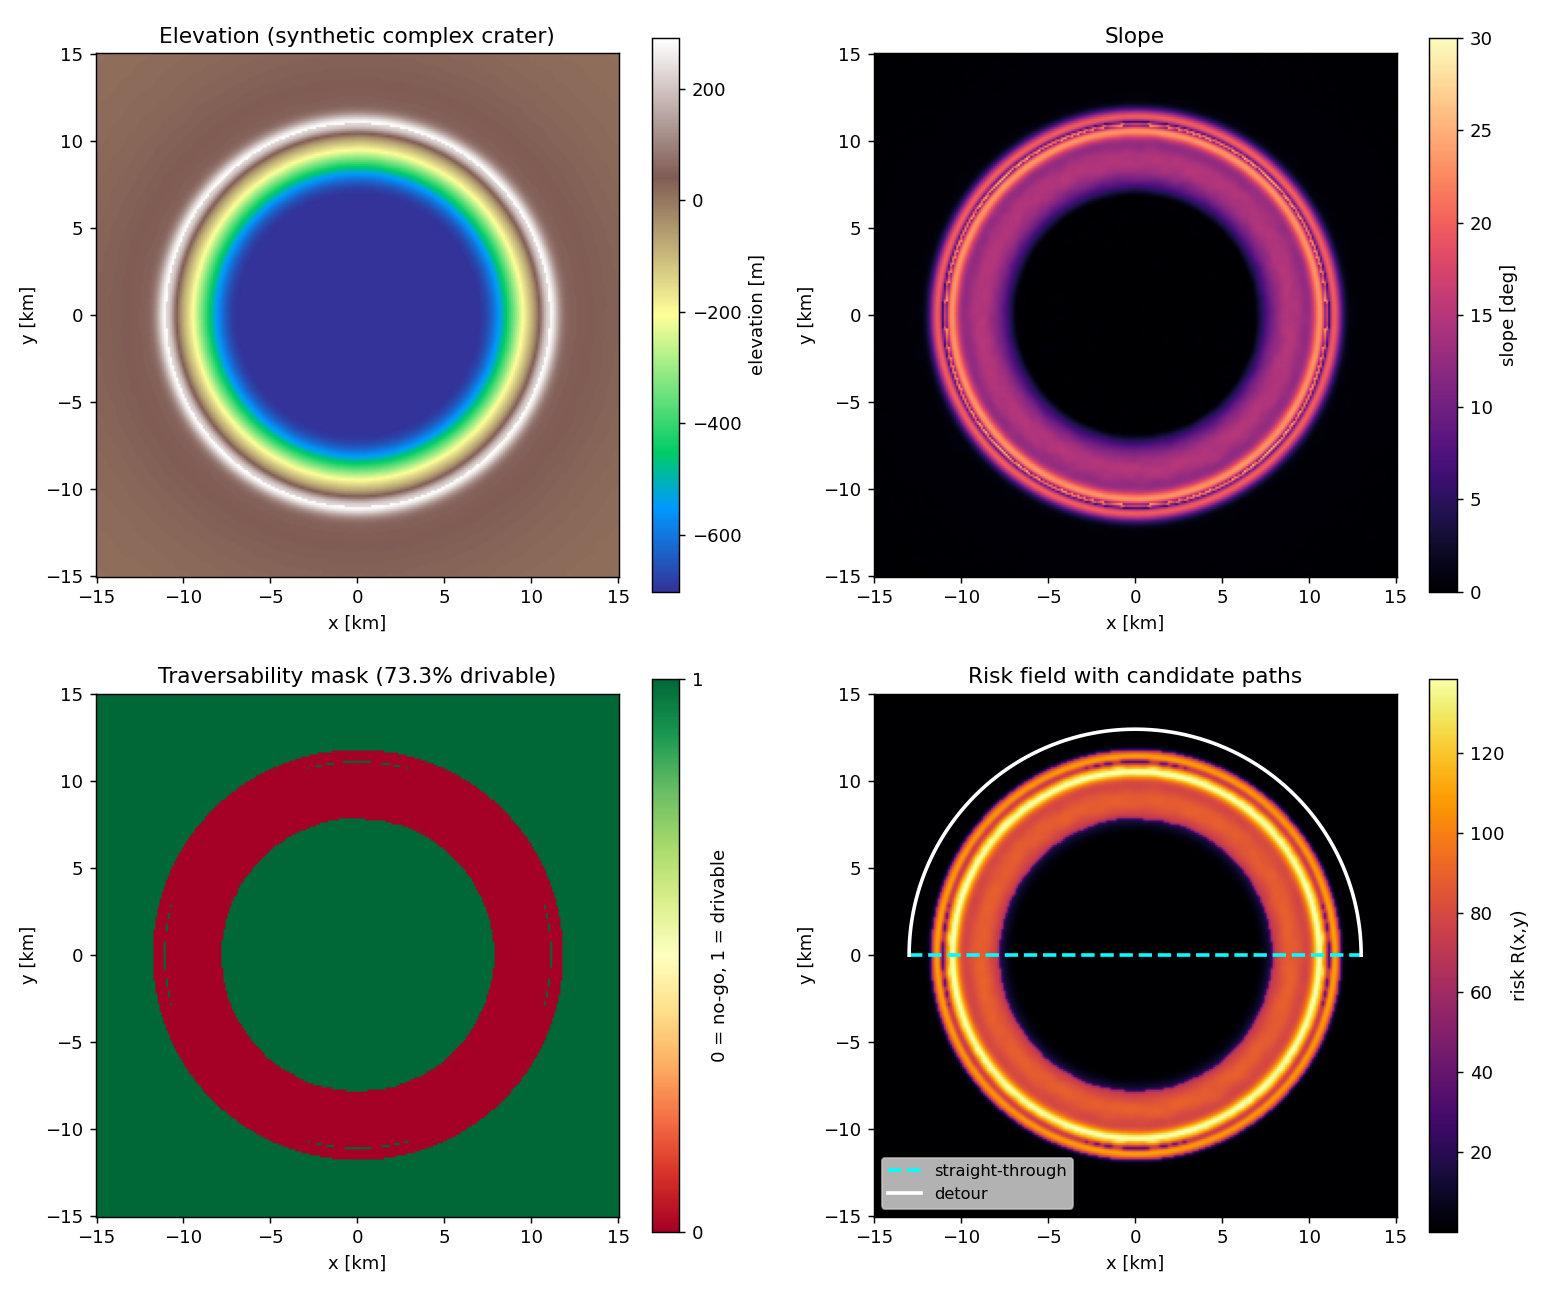
\includegraphics[width=0.95\linewidth]{terrain_validation.png}
\caption{Crater terrain validation. The elevation map is converted into slope, traversability, and risk layers. The traversability mask removes steep crater-wall and rim regions, while the continuous risk field discourages routes near hazardous terrain.}
\label{fig:terrain}
\end{figure}


\section{Results and Discussion}
The proposed planner--trajectory-generation pipeline successfully generated a lunar rover route from the prescribed start location to the goal across cratered terrain. As shown in Fig.~\ref{fig:terrain}, the terrain module converts the elevation map into traversability and risk information that marks steep crater-wall and rim regions as undesirable. A$^\ast$ then produced a high-level route around the high-risk terrain, and the trajectory stage produced a time--energy trajectory along this route while enforcing the implemented rover dynamics, power limits, battery bounds, and rate constraints.

The terrain pipeline provides a useful validation of the benchmark before trajectory optimization. The synthetic crater has elevation ranging from approximately \SI{-702}{m} to \SI{291}{m}, and the slope field reaches approximately $25.6^\circ$ inside the wall annulus. The traversability mask leaves approximately $73.3\%$ of the map drivable: the crater floor and surrounding plains remain available, while the steep wall and rim annulus are excluded or assigned high risk. This confirms that the terrain layer separates the hazardous crater boundary from the lower-risk regions available for routing.

The global planner then verifies that the risk field induces the intended distance--risk tradeoff. With $w_{\mathrm{risk}}=10$, A$^\ast$ returns a 312-waypoint route with length approximately \SI{43.25}{km}. Its path-integrated terrain risk is approximately $9.99\times10^2$, compared with $7.20\times10^5$ for the straight-line baseline. Thus, the planner reduces terrain exposure by roughly $721\times$ at a $1.66\times$ increase in path length. This confirms that the terrain cost discourages short but hazardous crossings and instead produces a feasible warm start for the trajectory-generation stage.

\begin{table}[t]
\centering
\caption{Effect of terrain-risk weight on global planner output.}
\label{tab:risk_weight_sweep}
\begin{tabular}{ccc}
\toprule
Risk weight $w_{\mathrm{risk}}$ & Length (km) & Path-integrated risk \\
\midrule
0   & 39.97 & $7.26\times10^5$ \\
1   & 41.73 & $1.42\times10^3$ \\
10  & 43.25 & $9.99\times10^2$ \\
100 & 56.21 & $3.39\times10^2$ \\
\midrule
Straight-line baseline & 26.08 & $7.20\times10^5$ \\
\bottomrule
\end{tabular}
\end{table}

Table~\ref{tab:risk_weight_sweep} shows the planner tradeoff more directly. Increasing $w_{\mathrm{risk}}$ increases the route length but decreases path-integrated risk, producing a clear distance--risk Pareto trend. This behavior is consistent with the planner edge cost, which combines geometric distance with an approximation of terrain-risk exposure.

The full-route trajectory covers approximately \SI{42.0}{km} and reaches the goal in approximately \SI{152135}{s}, or \SI{42.3}{h}. The trajectory remains battery-feasible throughout the traverse: starting from \SI{5.0}{MJ}, the rover finishes with approximately \SI{2.33}{MJ} of remaining battery energy. These results show that the navigation objective was achieved for the benchmark terrain and simplified rover model.

The panels in Fig.~\ref{fig:main_results} separate the geometric, energy, and command behavior of the returned solution. Figure~\ref{fig:trajectory} shows that the trajectory follows the smoothed A$^\ast$ route while avoiding the high-risk terrain identified by the terrain layer. Figure~\ref{fig:battery} shows that battery energy remains within the imposed bounds. Figure~\ref{fig:speed} shows that the solution remains within the rover speed limit and uses a mostly steady low-speed traverse over the long route. Figure~\ref{fig:power} shows modeled power demand over time. Figure~\ref{fig:heading} shows the heading command required to follow the curved route.

The time--energy objective is reflected in the long-duration, low-speed solution. This lets the trajectory-generation stage balance traversal time, energy use, and feasibility constraints. The battery decrease is smaller than the integral of modeled power demand because the battery model subtracts the constant generation offset. The nearly constant power trace is mainly a consequence of the reduced-order energy model, where power is dominated by the baseline load and low-order motion-dependent terms. It should therefore be interpreted as an energy-accounting result rather than a high-fidelity prediction of terrain-dependent electrical load.

Overall, the experiment demonstrates that the proposed decomposition is effective for the intended benchmark. The global planner provides terrain feasibility over a hazardous map, and the trajectory stage returns a dynamically consistent, battery-feasible route to the goal. This supports the use of a planner-plus-trajectory-generation architecture for long-horizon rover navigation over cratered lunar terrain.




\begin{figure}[h]
\centering
\begin{subfigure}{0.48\linewidth}
\centering
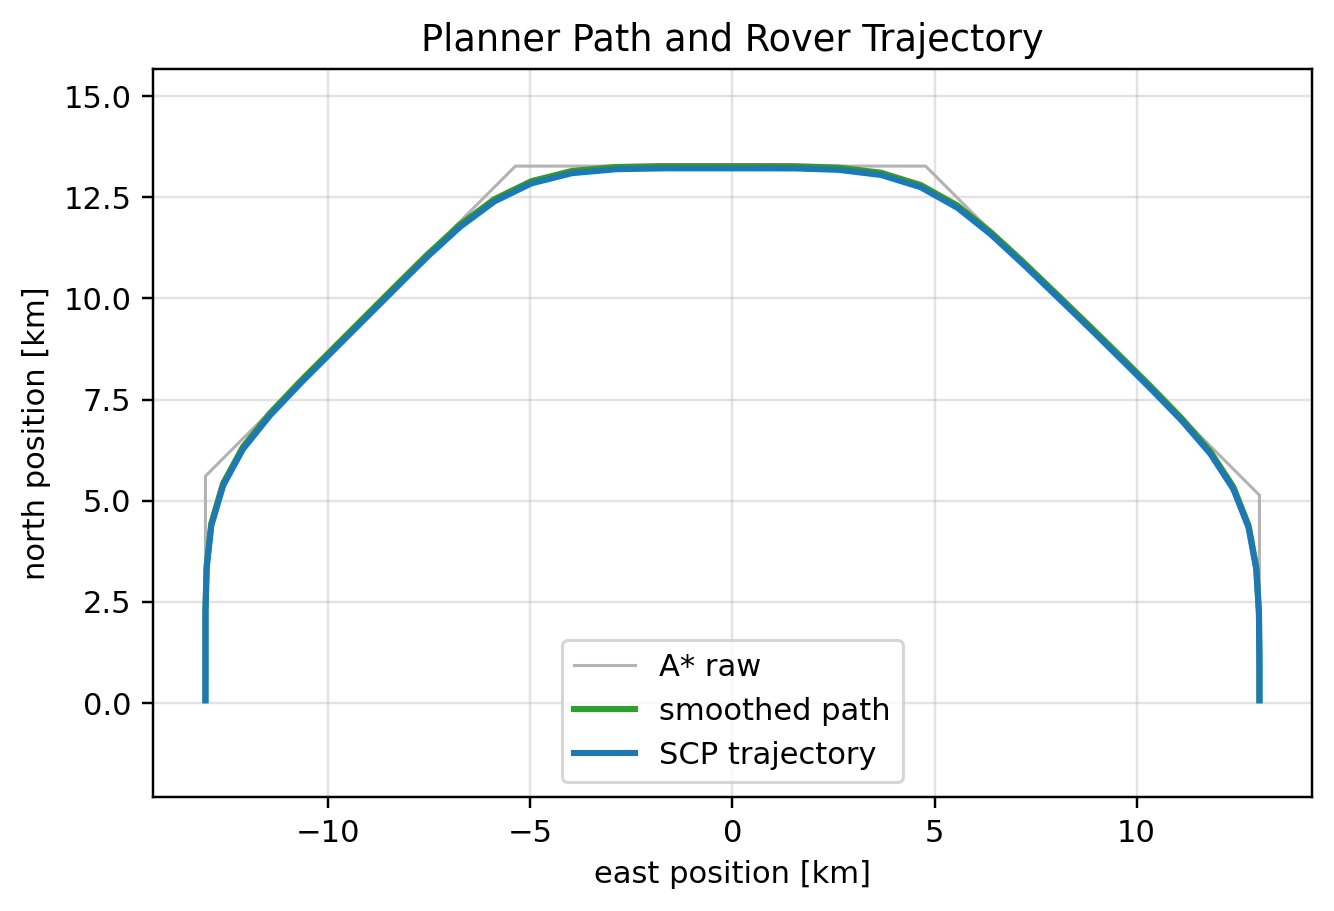
\includegraphics[width=\linewidth]{trajectory.png}
\caption{Planner path and trajectory.}
\label{fig:trajectory}
\end{subfigure}
\hfill
\begin{subfigure}{0.48\linewidth}
\centering
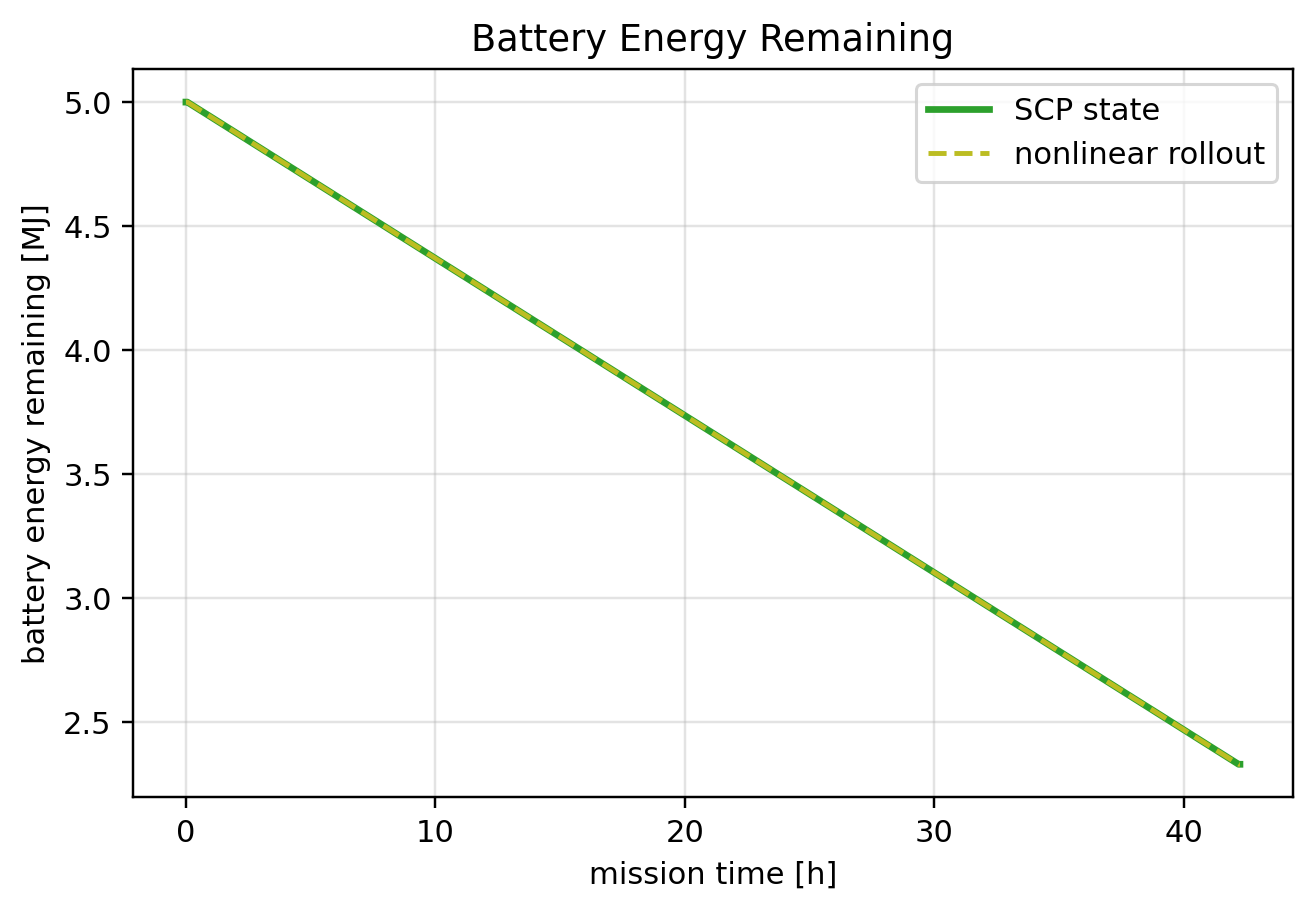
\includegraphics[width=\linewidth]{battery_energy_hours.png}
\caption{Battery energy.}
\label{fig:battery}
\end{subfigure}

\vspace{0.5em}
\begin{subfigure}{0.48\linewidth}
\centering
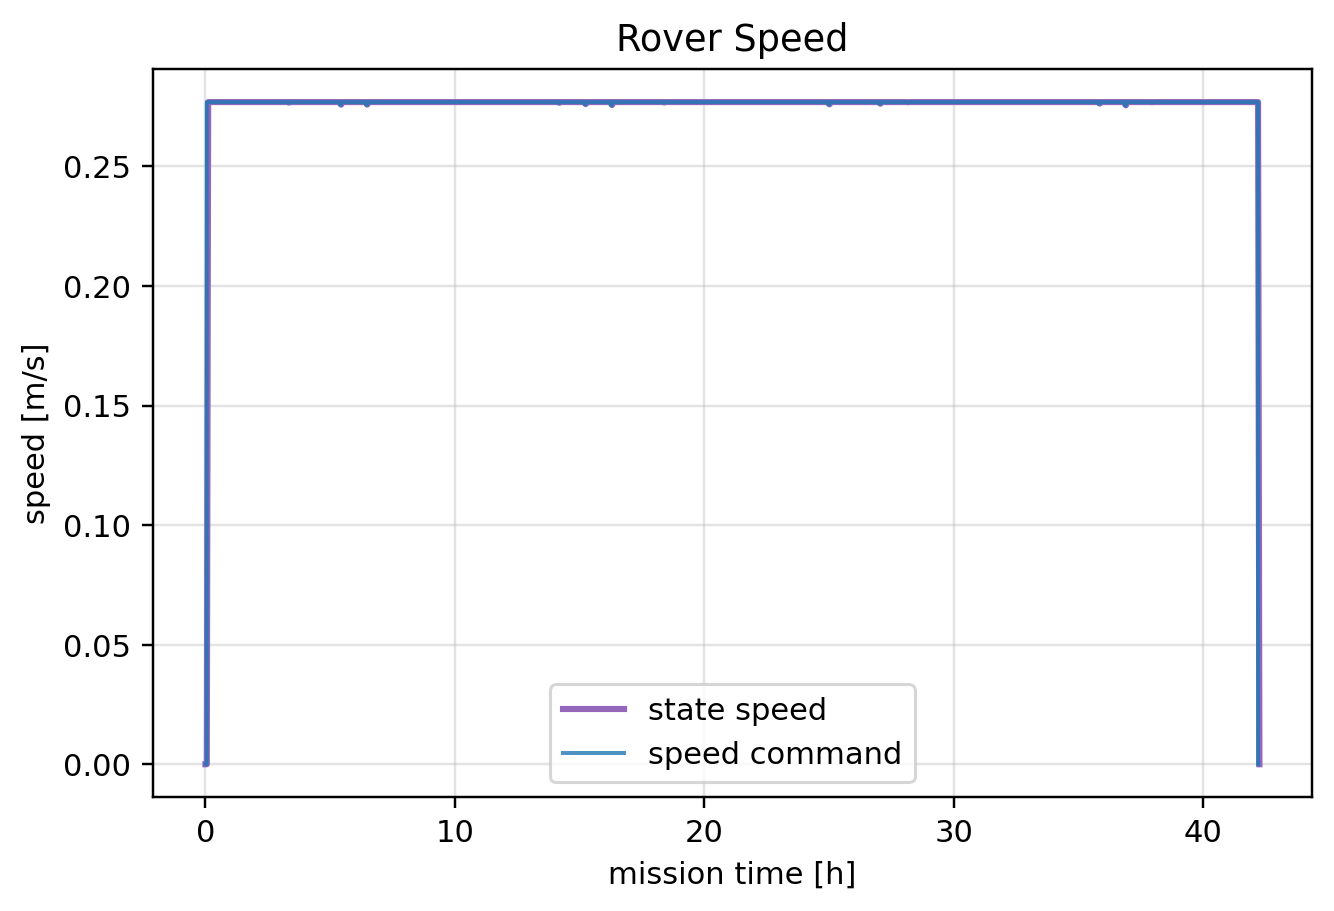
\includegraphics[width=\linewidth]{speed_hours.png}
\caption{Rover speed.}
\label{fig:speed}
\end{subfigure}
\hfill
\begin{subfigure}{0.48\linewidth}
\centering
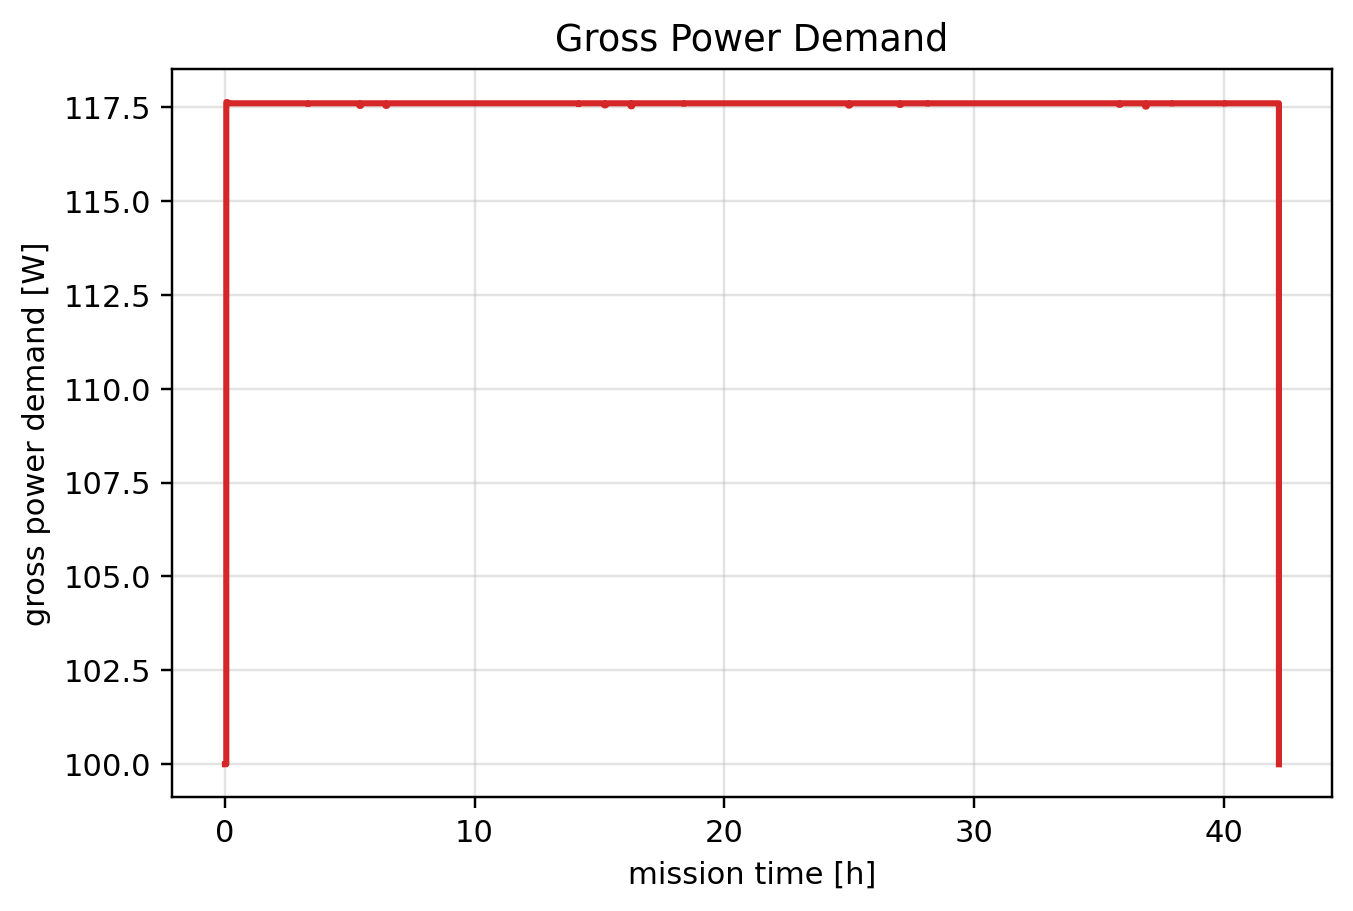
\includegraphics[width=\linewidth]{power_hours.png}
\caption{Power consumption.}
\label{fig:power}
\end{subfigure}

\begin{subfigure}{0.48\linewidth}
\centering
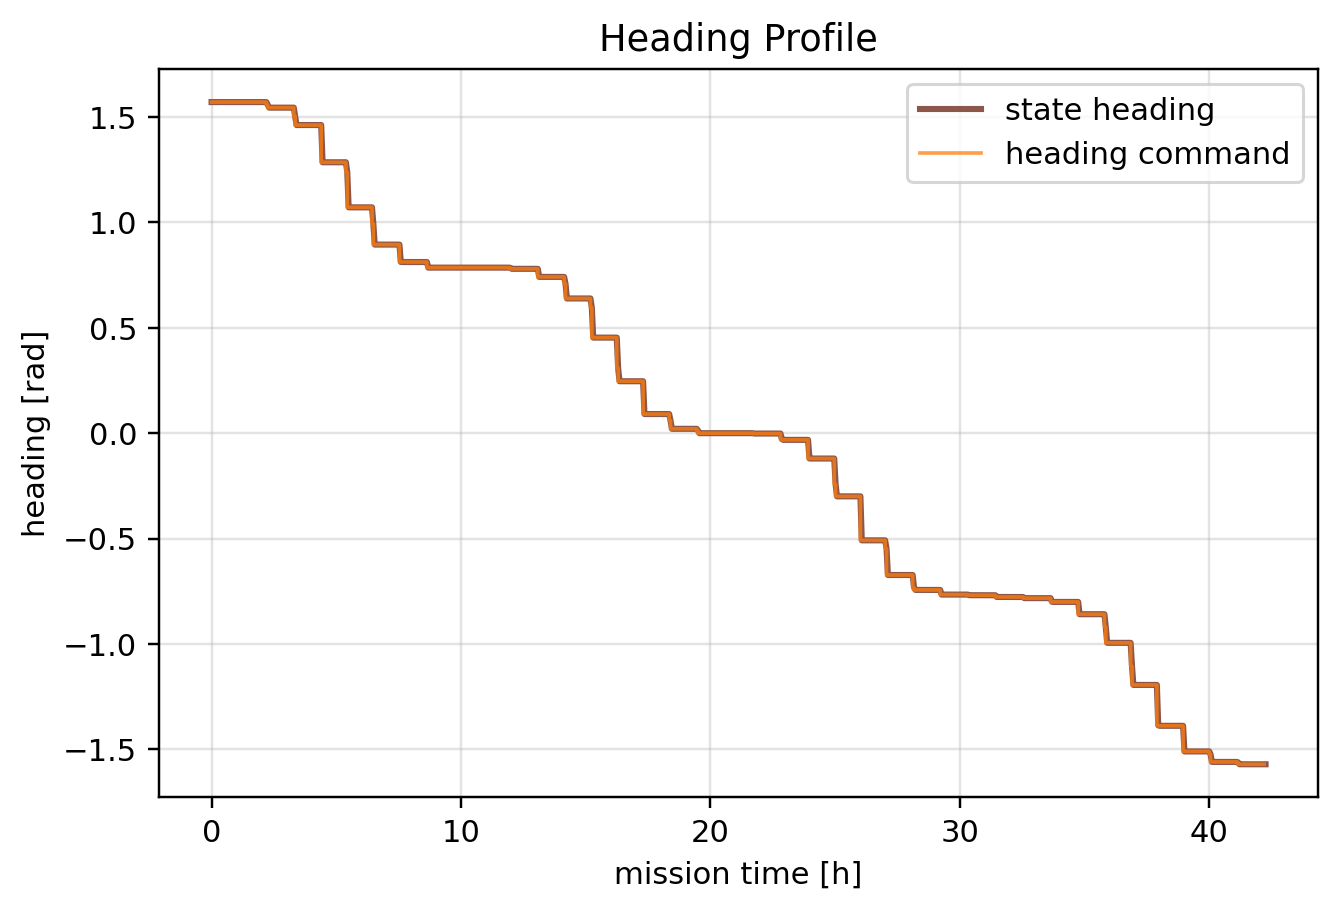
\includegraphics[width=\linewidth]{heading_hours.png}
\caption{Commanded heading.}
\label{fig:heading}
\end{subfigure}
\caption{Results for the full lunar-rover benchmark.}
\label{fig:main_results}
\end{figure}

\section{Conclusion}
This project implemented a lunar rover navigation pipeline that combines terrain-aware global planning with SCP-based trajectory-generation. The terrain module produces a traversability map and risk field, the A$^\ast$ planner generates a feasible high-level route, and the rover model converts that route into a dynamically consistent time--energy trajectory. The formulation permits segment final time to vary rather than imposing a fixed nominal traversal speed.

The benchmark result shows that the pipeline achieves the main objective of lunar rover navigation across cratered terrain. The returned route covers approximately \SI{42.0}{km}, reaches the goal in approximately \SI{42.3}{h}, satisfies the nonlinear rover dynamics to numerical precision, and remains battery-feasible under the implemented energy model. Thus, the proposed method successfully produces a feasible time--energy trajectory for the simplified rover model and mission scenario considered in this work.

The main limitations are associated with model fidelity and the prototype SCP implementation. The energy model uses a simplified power representation with a constant generation offset and does not model active recharging, spatially varying solar incidence, slip, sinkage, or detailed wheel--soil interaction. In addition, the SCP merit-filtering and trust-region logic are conservative in the current implementation, so further tuning is needed to make the local refinement stage consistently accept improving trajectory updates.

Future work should couple terrain and trajectory optimization more tightly by adding continuous terrain-risk or terrain-resistance terms directly inside the trajectory optimizer. The energy model should also be extended to support active recharge, spatially varying solar generation, terrain-dependent resistance along the route, and more realistic terramechanics. Finally, evaluating the method on a larger set of LOLA-derived lunar terrain maps would provide a more representative assessment for south-pole mission planning~\cite{nasa_lola,moon_sokolov}.


\section{Contributions}
Martin Zhou implemented the terrain pipeline, global planning stack, and the planner/SCP integration used in the final benchmark. Sebastian Martinez implemented and refined the rover dynamics model, the JAX-based SCP linearization path, and the supporting trajectory optimization tests. Both authors contributed to the paper writing and revision.

\bibliography{sample}

\end{document}
